\documentclass{article}

\usepackage[utf8]{inputenc}
\usepackage[T1]{fontenc}
\usepackage{microtype}
\usepackage[spanish]{babel}

\usepackage{newspaper}

\date{26 de octubre de 2017}
\currentvolume{7}
\currentissue{42}

\SetPaperName{La Didáctica}
\SetHeaderName{La Didáctica}

\SetPaperLocation{Ciudad Universitaria}
\SetPaperSlogan{``No hay otra elección que comprometerse''}
\SetPaperPrice{Para todas y todos}

\usepackage{graphicx}
\usepackage{float}
\usepackage{multicol}
\usepackage{picinpar}
\usepackage{newspaper-mod}

\begin{document}
\maketitle

\begin{multicols*}{3}

\byline{¡Genética, tovarish!}{Listunovna Semyonovna}
 
\begin{window}[0,l,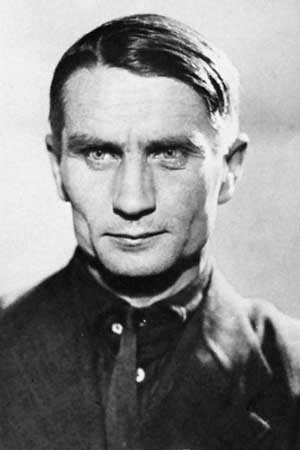
\includegraphics[width=1.0in]{Trofim_Lysenko_portrait.jpg},\centerline{\small{Trofym Lysenko}}] Trofym Lysenko nació en el seno de una familia de campesinos en Ucrania y hacia 1925, el hoy \textit{<<notorio>>} horticultor, comenzó a trabajar en los efectos de las bajas temperaturas en el desarrollo de plantas de cultivo. Sus experimentos con cereales y algodón fueron sorprendentes: algunos tratamientos a temperaturas bajas en semillas húmedas podían cambiar las propiedades fisiológicas de las plantas. En 929, las afirmaciones de Lysenko de poder incrementar el rendimiento de las cosechas eran poderosamente seductoras para una Rusia que sufría de sequías y hambrunas.   
\end{window}

Con asombrosa rapidez y de la mano de científicos de renombre y de los líderes del Partido Comunista, Lysenko subió en la escalera gubernamental y tuvo la posibilidad de probar sus teorías a gran escala: jamás pudo aumentar el rendimiento de las cosechas y, para no perder el favor del gobierno y su renombre (como mínimo), se vió forzado a falsificar sus resultados.

Los ardides de Lysenko continuaron de forma ininterrumpida y casi sin intervención hasta 1965. De hecho, Lysenko ganó varias medallas doradas del Premio Stalin y fué galardonado siete veces con la Orden de Lenin, el mayor honor soviético. Y he aquí el primer dato que pretendo traer a nuestra comprensión de la ciencia: Lysenko se proclamó en contra de la genética de Mendel, la teoría de la evolución darwiniana y el concepto de gen; se trataba de \textit{``la biología burguesa''} que encima consideraba incorrecta a las teorías de Lysenko. Pero quizás, más sorprendentemente humano aún, sea el hecho de que mientras los trabajos especializados de científicos  e historiadores occidentales aseguran que las ideas de Lysenko tuvieron graves repercusiones sobre las cosechas soviéticas, ninguno de esos trabajos expone datos concretos al respecto. Entonces, ¿con qué tipos de hipótesis trabajamos al construir modelos de la realidad?. ¿Con qué tipos de argumentos decimos que \textit{el otro está <<equivocado>>}?  
\closearticle


\byline{Rayos curativos}{Carmo Flannán}

\begin{window}[0,l,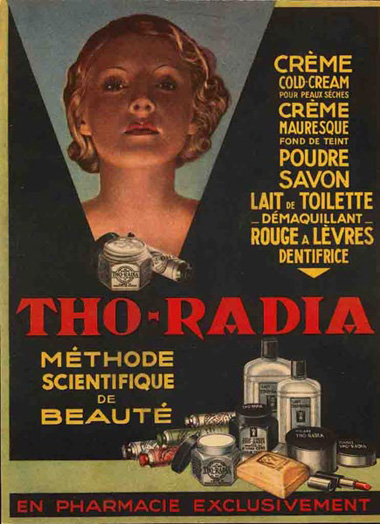
\includegraphics[width=1.0in]{tho-radia_cream.jpg},\centerline{\small{Crema para manos}}] El choco-radio \textit{Radium Schokolade}, el dispenser de agua con recubrimiento de radio \textit{Revigator}, y el jabón y dentífrico \textit{Tho-Radia} son sólo algunos de los productos comerciales radiactivos de principios del siglo XX. Incluso, si se busca con cuidado, se pueden encontrar apliques para el tratamiento de la impotencia.   
\end{window}

El descubrimiento del elemento químico radio por parte de Marie Slodowska-Curie y su esposo Pierre fue durante muchos años la panacea medicinal con la que soñaban los alquimistas de la Edad Media. Para situarnos en la vorágine: a un mes del descubrimiento de los Rayos X, éstos ya se habían utilizado para tratar tumores en pacientes con cáncer, y los rayos que emanaba el radio eran considerablemente más potentes que los Rayos X. En pocos años, el radio pasó del laboratorio a la fábrica y de curiosidad física a producto comercializable. ¿Quién iba a difundir la idea de que la utilización del radio era peligrosa? Después de todo, los rayos del radio podían destruir tumores.

Científicos y científicas como la mismísima Marie Slodowska-Curie, haciendo uso de su rol como actores sociales, fomentaban el uso milagroso del radio y sus beneficios. De a poco, investigación y experiencia mediante, se comprendió el horror de la realidad: el radio actúa sobre las células vivas, y no sólo sobre las tumorales. El asunto es sumamente complejo, porque científicos y científicas como Marie Slodowska-Curie minimizaron rápidamente los nefastos efectos del radio sobre la salud humana como simples \textit{<<efectos secundarios>>}. Estas historias nos suscitan sentimientos encontrados: queremos culpar a esta ciencia y sus desarrolladores, pero también reconocemos los resultados científicos hoy en día (por ejemplo, la radioterapia oncológica). ¿Con qué ojos miramos los científicos del pasado?. Alguna vez he escuchado la frase \textit{``las armas no matan, matan las personas''}, pues quizás sea correcto que nos preguntemos: ¿bajo qué concepciones podemos decir que la ciencia y los científicos son sujetos distintos?  

\closearticle

\byline{{Duelo a los dualismos}\\[10pt] Extracto del libro cuerpos sexuados}{Anne Fausto-Sterling}

\begin{window}[0,l,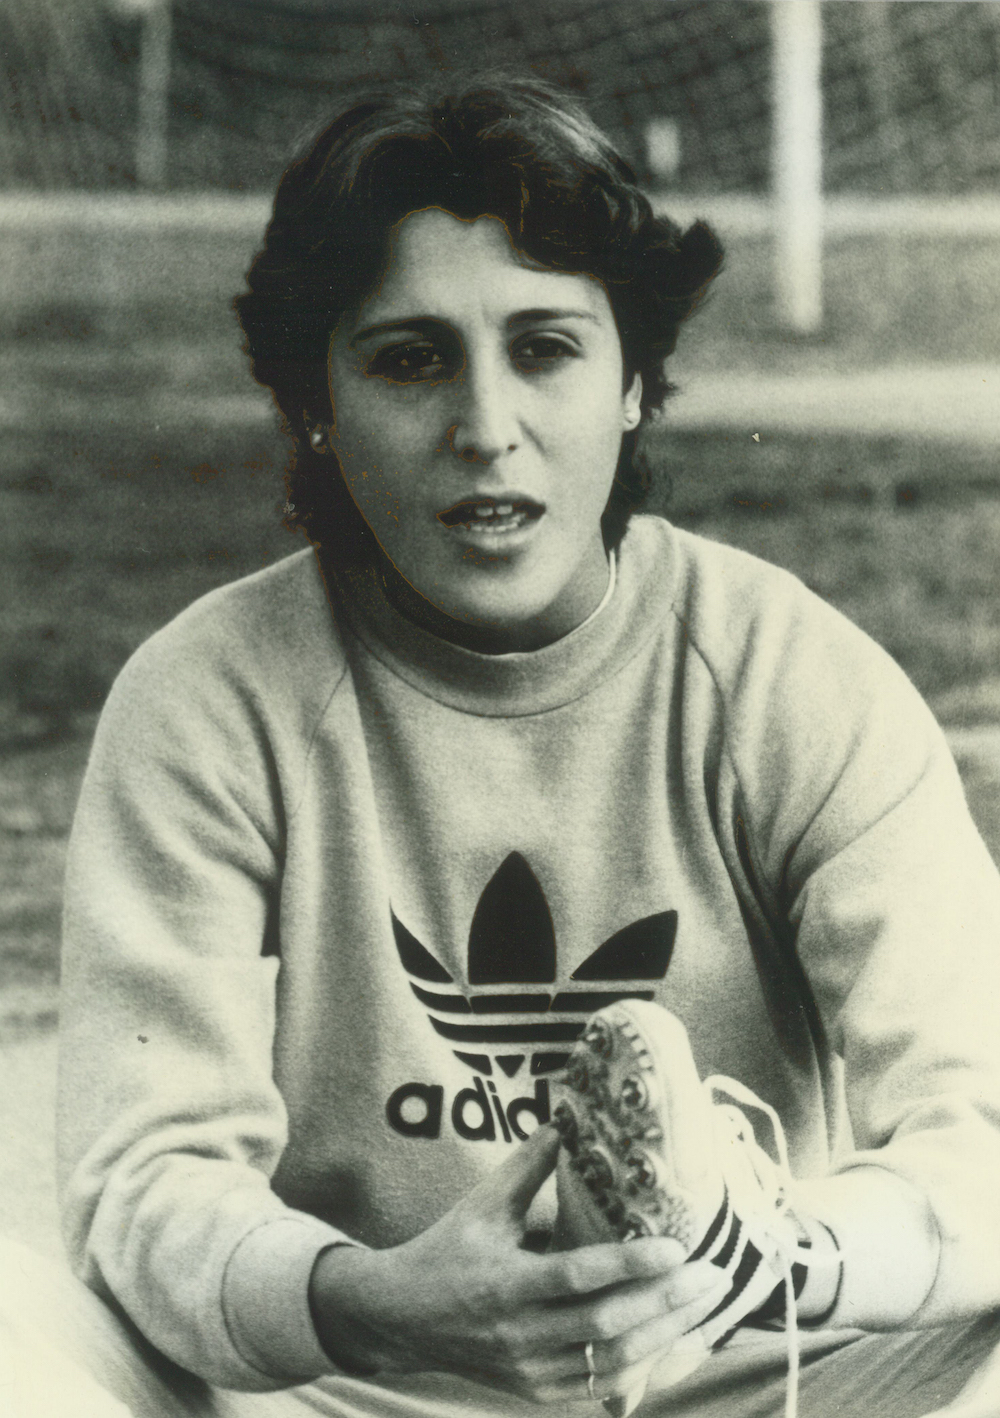
\includegraphics[width=1.0in]{patinio.jpg},\centerline{\small{María Patiño}}] Con las prisas y emoción de la partida hacia los juegos olímpicos de 1988, María Patiño, la mejor vallista española, olvidó el preceptivo certificado médico que debía dejar constancia, para seguridad de las autoridades olímpicas, de lo que parecía más que obvio para cualquiera que la viese: que era una mujer. [...] Patiño sólo tenía que informar al \textit{<<centro de control de feminidad>>} , raspar unas cuantas células de la cara interna de su mejilla, y todo estaría en orden\ldots O así lo creía.
\end{window}

Cuando se dirigía al estadio olímpico para su carrera, los jueces de pista le dieron la noticia: no había pasado el control de sexo. Puede que pareciera una mujer, que tuviera la fuerza de una mujer, y que nunca hubiera tenido ninguna razón para sospechar que no lo fuera, pero los exámenes revelaron que las células de Patiño tenían un cromosoma Y, y que sus labios vulvares ocultaban unos testículos. Es más, no tenía ovarios ni útero. De acuerdo con la definición del COI [Comité Olímpico Internacional], Patiño no era una mujer. En consecuencia, se le prohibió competir con el equipo femenino español.

[...] Patió decidió plantar cara al COI. <<Sabía que era una mujer>>, insistió a un periodista, <<a los ojos de la medicina, de Dios y, sobre todo, a mis propios ojos>>. [...] Patiño se sometió a exámenes médicos de sus cinturas pélvica y escapular <<con objeto de decidir si era lo bastante femenina para competir>>. Al cabo de dos años y medio, la IAAF (International Amateur Athletic Federation) la rehabilitó, y en 1992 se reincorporó al equipo olímpico español, convirtiéndose así en la primera mujer que desafiaba el control de sexo para atletas olímpicas. A pesar de flexibilidad del IAAF, sin embargo, el COI se mantuvo en sus trece: si la presencia de un cromosoma Y no era el criterio más científico para el control de sexo, entonces había que buscar otro. [...] Pero, ¿por qué le preocupa tanto al COI el control de sexo? (\textit{Agregado por el editor: ¿qué posición tomamos al delegar el <<control de sexo>> a la ciencia?})

\closearticle

\byline{Aristóteles el biólogo}{Alberto Fuertes}

Una de las facetas poco recordadas del famoso filósofo fue la de conocedor y catalogador de plantas y animales, porque en esa época o eras todo o eras un esclavo. Sus obras de botánica y zoología fueron recopiladas y ampliadas durante la Edad Media, y se convirtieron en los \textit{<<herbarios y bestiarios>>}; obras donde se mencionaban y describían animales, plantas y minerales, resaltando propiedades muchas veces fantasiosas. En esas obras que de alguna manera ampliaron los saberes prácticos sobre la flora y fauna local, se fueron perdiendo información sobre especies africanas, asiáticas y mediterráneas estudiadas en la biología de la antigüedad.

Los bestiarios medievales reflejan una concepción de la ciencia en la que esta debía estar al servicio de la fe. La misión de la ciencia se expresó en una repetición del saber tradicional con muy escaso aporte de la observación directa: el contenido cobró un carácter simbólico al que se agregó una \textit{moraleja cristianizante}. Aquí se presenta un texto de un bestiario, donde se observa que a los animales reales se le atribuían comportamientos imaginarios:

\begin{window}[2,r,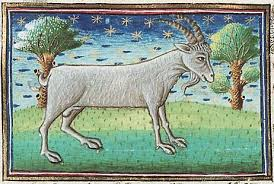
\includegraphics[width=1.0in]{images.jpg},\centerline{\small{Cabra medieval}}] \textit{``La cabra salvaje (Caprea) tiene las siguientes particularidades: que va subiendo y subiendo mientras pasta, que escoge las buenas yerbas de entre las malas gracias a su agudeza de su vista, que rumia estas yerbas y que, si es herida, corre hacia la planta díctamo (orégano), alcanza la cual se cura.''}
\end{window}

Esta historia nos muestra cómo las concepciones de ésa época forman parte de la concepción de ciencia. ¿Es la ciencia tan distinta de la \textit{concepción de ciencia}? ¿Cuáles serán (si las hay) concepciones de época en \textit{nuestra} ciencia moderna?

\closearticle

\byline{Atibiótico histórico}{Laura Elorrieta}

\begin{window}[0,l,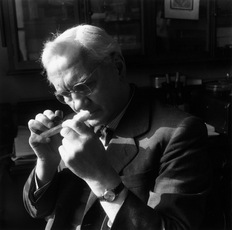
\includegraphics[width=1.0in]{fleming.jpg},\centerline{\small{Alexander Fleming}}] La historia más divulgada cuenta que, en 1928, cuando Alexander Fleming volvía de sus vacaciones a su desordenada mesa de laboratorio en St. Mary's Hospital, ni se imaginaba que allí lo esperaba el premio Nobel de 1945. En una de las placas de petri donde Fleming estudiaba ciertas bacterias estaba creciendo \textit{moho}, un hecho bastante común. Pero lo que sorprendió al médico fue que \textit{ése} moho en particular, parecía estar previniendo el desarrollo normal de la bacteria. La historia otra vez nos cuenta que Fleming logró \textit{descubrir} que el moho también podía curar enfermedades infecciosas. Ese moho se convirtió en la \textit{penicilina}, el primer antibiótico hecho y derecho 
\end{window}

Lo que la historia ``se olvida'' de contarnos es que Fleming carecía de recursos de laboratorio y de la formación en química necesaria para llegar desde el moho hasta la penicilina. Esa tarea recayó en los doctores Howard Florey y Ernst Chain, quien había huído de la Alemania nazi; ambos trabajaron juntos sobre lo hecho y publicado por Fleming, describiendo la composición química y usos terapéuticos de la penicilina.

El \textit{descubrimiento} siguió de la forma usual: luego de muchas pruebas en placas de petri, se hicieron pruebas en ratones y otros animales, luego se encontró a algún sujeto dispuesto a probar suerte. En 1940, Albert Alexander de 48 años, se había cortado la cara trabajando en su jardín de rosas y su infección fue tratada con penicilina. El tratamiento parecía ser exitoso, pero Florey y Chain se quedaron sin penicilina y Alexander falleció. El primer caso exitoso llegaría recién en 1942. Parece ser que la historia de la ciencia es tan humana como la ciencia misma, y cada tanto se toma alguna \textit{licencia poética}. ¿Cuál será la utilidad de \textit{reescribir} la historia de la ciencia? ¿Se toma una posición particular al hacerlo?

\closearticle

\headline{ Como decía Althusser}

\textbf{\textit{``En la batalla que es la filosofía todas las técnicas de la guerra, incluidos el saqueo y el camuflaje, están permitidas.''}}

\begin{figure}[H]
	\centering	
    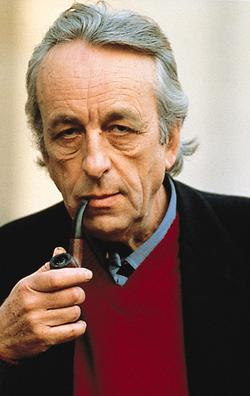
\includegraphics[width=.4\columnwidth]{Althusser}
\end{figure}

\closearticle
\end{multicols*}

\end{document}